\documentclass{beamer}
\usepackage[spanish]{babel}
\usepackage{graphicx}
\usepackage{xcolor}
\usepackage{latexsym}
\usepackage{amsmath}
\usepackage{amssymb}
\usepackage{multicol}
\usepackage{tikz}

\usetheme{Boadilla}

\newtheorem{Teorema}{Teorema}

\definecolor{myblue}{RGB}{80, 69, 190} 

\setlength{\parskip}{0.1cm}

\newcommand{\myref}[2]{
    {\color{blue}\href{#1}{#2}}
}

\newcommand{\mytitle}[4]{
    \centering
    \vspace{0.1cm}
    
    {\Large \color{myblue} #1}

    \vspace{0.1cm}

    {\Large \color{myblue} #2}
    
    \vspace{0.5cm}
    
    {#3}
    
    \vspace{0.5cm}
    
    {\color{gray} #4}
    
    \vspace{0.5cm}
    
    {\today}
}

\newcommand{\estindc}[2]{
    \begin{frame}
        \frametitle{Índice}
        	\begin{enumerate}
            \setbeamercovered{transparent}
            \item <#1> The Future of the data storage in Particle Physics and Astronomy
            \item<#2> Fraud Detection in NoSQL Database Systems using Advanced Machine Learning
        \end{enumerate}
    \end{frame}
}

\title{Bases de datos NoSQL}
\author{Arroyo Joaquin \\ Belmonte Marina}

\begin{document}

\begin{frame}
    \mytitle
    {Bases de datos NoSQL}
    {Clase 3}
    {Arroyo Joaquin \\ Belmonte Marina}
    {Universidad Nacional de Rosario \\ Licenciatura en Ciencias de la Computación \\ Bases de Datos Avanzadas}
\end{frame}

\section{Resumen}
\begin{frame}
    \frametitle{Resúmen}

    \begin{itemize}
        \item Repaso de Modelos NoSQL

         
        
        \item Implementaciones de Modelos NoSQL

        \begin{itemize}
            \item Redis
            \item Apache HBase
            \item MongoDB
            \item Neo4j
        \end{itemize}

         
        
        \item Dos artículos que estudian el rendimiento de bases de datos SQL versus NoSQL en aplicaciones reales
    \end{itemize}
    
\end{frame}

\section{Estado Del Arte}

\estindc{1}{0}
\subsection{The Future of the data storage in Particle Physics and
Astronomy}
\section{Introducción}

\begin{frame}
    \frametitle{The Future of the data storage in Particle Physics and Astronomy - Introducción}

    \begin{itemize}
        \item Desarrollado por Julius Hřivnáč y Julien Peloton, investigadores de la Université Paris-Saclay, en el año 2024.

         
        
        \item Hace incapié en la combinación de bases de datos, en particular ``tabulares" (SQL o NoSQL) con Grafos, para el almacenado de datos astronómicos y de experimentos de física de partículas.

          

        \item Los experimentos de física de partículas y los telescopios de astronomía almacenan grandes cantidades de datos, principalmente en archivos simples en diversos formatos, con un uso limitado de bases de datos.
        
    \end{itemize}
    
\end{frame}

\begin{frame}
    \frametitle{The Future of the data storage in Particle Physics and Astronomy - Introducción}

    \begin{columns}
        \begin{column}{0.67\textwidth}
            Ilustran dicha combinación de  bases de datos con el proyecto FINK, uno de los brokers oficiales dentro del Observatorio Rubin y del Zwicky Transient Facility.
        \end{column}
        \begin{column}{0.3\textwidth}
            \centering
            
\includegraphics[width=1\textwidth]{images/fink_logo.png}
        \end{column}
    \end{columns}

    \vspace{0.15cm}

    Este proyecto utiliza \textbf{HBase} y \textbf{JanusGraph} para almacenar alertas:
    
    \begin{itemize}
        \item HBase almacena datos voluminosos.
        \item JanusGraph almacena información estructural.
    \end{itemize}
\end{frame}

\section{HEP y Grafos}

\begin{frame}
    \frametitle{The Future of the data storage in Particle Physics and Astronomy - HEP y Grafos}

    La motivación de proponer una combinación de bases de datos ``tabulares'' con grafos viene dada por las siguientes razones:

     
    
    \begin{itemize}
        \item En la Física de Alta Energía (HEP) el manejo de datos ha dependido durante mucho tiempo de estructuras de datos convencionales.

          
    
        \item Una parte significativa de estos datos exhiben características similares a grafos y carecen de un esquema rígido.

         

        \item Estos datos a menudo consisten en entidades conectadas a través de relaciones, lo que los hace poco adecuados para el almacenamiento en bases de datos relacionales.
    \end{itemize}
\end{frame}

\begin{frame}
    \frametitle{The Future of the data storage in Particle Physics and Astronomy - HEP y Grafos}

    Además esto es impulsado también por las propias desventajas que tienen las bases de datos de grafo:

     
    
    \begin{itemize}
        \item Inserción Lenta
        \item Manejo de Memoria Lento
        \item Creación de Aristas Anárquica
        \item Esquema Desconocido y Relaciones Caóticas
        \item Lenguajes de Consulta Avanzados
        \item etc. 
    \end{itemize}
\end{frame}

\begin{frame}
    \frametitle{The Future of the data storage in Particle Physics and Astronomy - Solución Híbrida}

    A la combinación que venimos mencionando la llaman ``Solución Híbrida'', la cuál ofrece lo mejor de ambos mundos al combinar las fortalezas de diferentes paradigmas de almacenamiento.

      

    \begin{itemize}
        \item Esta solución comienza almacenando datos no estructurados o en bruto en bases de datos tabulares.

          
        
        \item Se introduce el concepto de un grafo para expresar y gestionar estructuras de datos persistentes. Este representa relaciones y conexiones complejas dentro de los datos.

         

        \item Se conectan estos componentes detrás de una API común.
    \end{itemize}

     

    En esencia:

    \begin{itemize}
        \item Se aprovecha la eficiencia del almacenamiento tipo tabla
        \item y el poder expresivo de los grafos.
    \end{itemize}
    
\end{frame}

\section{Solución Híbrida}

\begin{frame}
    \frametitle{The Future of the data storage in Particle Physics and Astronomy - Solución Híbrida}

    Tres arquitecturas para conectar bases de datos tabulares y de grafos en una solución híbrida:
    
    \begin{center}
        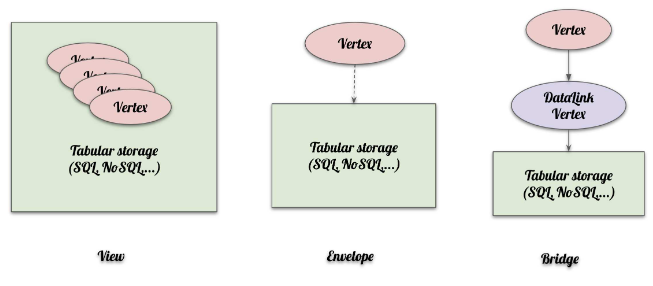
\includegraphics[width=0.75\textwidth]{images/multidb-1.png}
    \end{center}

\end{frame}

\begin{frame}
    \frametitle{The Future of the data storage in Particle Physics and Astronomy - Solución Híbrida}

    \begin{itemize}
        \item \textbf{Graph View:}

        \begin{itemize}
            \item Interpreta los datos tabulares existentes como vértices dentro de un grafo.

             
            
            \item Se agregan aristas adicionales al grafo para expresar relaciones estructurales entre estos vértices.
        \end{itemize}

         
    
        \item \textbf{Graph Envelope:}
        
        \begin{itemize}
            \item Mejora el concepto de un vértice agregando métodos adicionales para llenarlo desde un almacenamiento tabular externo.

             
            
            \item Mantener la consistencia entre los datos puede ser complicado.
        \end{itemize}

         

        \item \textbf{Bridge:} 
        
        \begin{itemize}
            \item Se crea de un tipo especial de \textbf{Vértice de Enlace de Datos} que representa relaciones con datos externos almacenados en cualquier tipo de sistema de almacenamiento.

             
                
            \item Estos vértices pueden estar conectados a cualquier otro vértice en el grafo, formando efectivamente puentes hacia fuentes de datos externas.
        \end{itemize}
    \end{itemize}

\end{frame}

\section{FINK}

\begin{frame}
    \frametitle{The Future of the data storage in Particle Physics and Astronomy - FINK}

    \begin{itemize}
        \item El proyecto FINK es uno de los brokers oficiales dentro del Observatorio Rubin y del Zwicky Transient Facility.

         

        \item El observatorio Rubin generará 10 millones de alertas cada noche, lo que equivale a aproximadamente 1 terabyte de datos de alerta con alrededor de 20 terabytes de datos de imagen.

         

        \item FINK está recibiendo y analizando los datos del Zwicky Transient Facility, el cuál desde 2019 está enviando en promedio 200,000 alertas por noche, las cuáles se procesan y distribuyen en tiempo real.
    \end{itemize}
    
\end{frame}

\begin{frame}
    \frametitle{The Future of the data storage in Particle Physics and Astronomy - FINK}

    \begin{itemize}
        \item Un aspecto esencial de FINK es la presencia de enlaces de datos que conectan los datos en JanusGraph con los datos correspondientes en HBase. 

         
        
        \item Estos enlaces de datos sirven como puentes entre los datos estructurados y orientados a grafos y los datos en bruto y tabulares almacenados en HBase.

         
        
        \item Esta combinación forma un sistema robusto de gestión de datos dentro del sistema, lo que permite un almacenamiento, organización y recuperación eficientes de los datos de alerta.
    \end{itemize}

\end{frame}

\begin{frame}
    \frametitle{The Future of the data storage in Particle Physics and Astronomy - FINK}

   \begin{figure}[H]
        \centering
        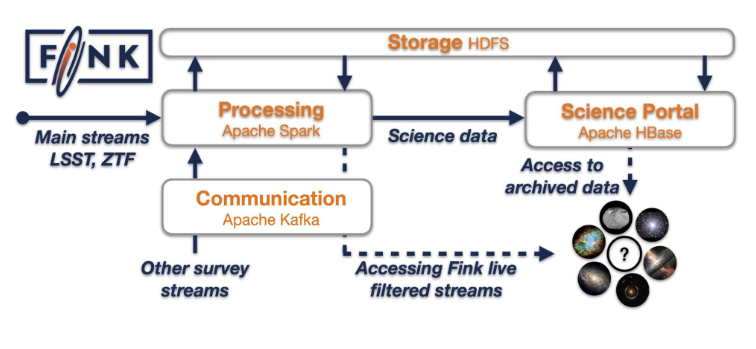
\includegraphics[width=0.9\textwidth]{images/multidb-2.png}
        \caption{La arquitectura del broker FINK.}
        \label{multidb-2}
    \end{figure}
    
\end{frame}

\begin{frame}
    \frametitle{The Future of the data storage in Particle Physics and Astronomy - Conclusiones}

    \begin{itemize}
        \item Se destaca la importancia de estructurar los datos de manera efectiva en el contexto de la Física de Altas Energías y las ventajas de utilizar soluciones de almacenamiento híbridas.

         
        
        \item Las soluciones de almacenamiento híbridas combinan la expresividad y flexibilidad de las bases de datos de grafos con el rendimiento y la simplicidad del almacenamiento tabular, proporcionando lo mejor de ambos mundos.

         

        \item Las bases de datos híbridas pueden mejorar la forma en que se manejan los datos en experimentos de HEP.
    \end{itemize}
    
\end{frame}

\estindc{0}{1}
\subsection{Fraud Detection in NoSQL Database Systems using Advanced Machine Learning}
\begin{frame}
    \frametitle{Fraud Detection in NoSQL Database Systems using Advanced Machine Learning}

    \begin{itemize}
        \item Autor: Tamilselvan Arjunan.
         
        \item Publicado en: International Journal of Innovative Science and Research Technology.
        \item Fecha: Marzo 2024.
         
        \item Análisis de vulnerabilidades en MongoDB y Cassandra.
         
        \item Propuesta de algoritmos de aprendizaje automático.
    \end{itemize}
\end{frame}

\begin{frame}
    \frametitle{Fraud Detection in NoSQL Database Systems using Advanced Machine Learning - Problemas de Seguridad en NoSQL}
    \begin{itemize}
        \item Esquemas Dinámicos.
         
        \item Falta de Control de Acceso.
         
        \item Consistencia Eventual.
         
        \item Datos Desnormalizados.
         
        \item Configuraciones Inseguras por Defecto.
    \end{itemize}
\end{frame}

\begin{frame}
    \frametitle{Fraud Detection in NoSQL Database Systems using Advanced Machine Learning - Soluciones Propuestas}
    \begin{itemize}
        \item Monitoreo en Tiempo Real.
         
        \item Algoritmos de Aprendizaje Automático:
        \begin{itemize}
            \item Modelos Supervisados.
             
            \item Técnicas No Supervisadas.
             
            \item Métodos en Línea.
             
        \end{itemize}
        \item Ingeniería de Características.
         
        \item Sistema Híbrido de Detección.
         
        \item Aprendizaje Adversarial.
         
        \item Implementación y Despliegue.
    \end{itemize}
\end{frame}

\begin{frame}
    \frametitle{Fraud Detection in NoSQL Database Systems using Advanced Machine Learning - Conclusiones}
    \begin{itemize}
        \item Las técnicas avanzadas de aprendizaje automático mejoran la seguridad.
         
        \item Mejorar los mecanismos de control de acceso y autenticación permitirían reducir la superficie de ataque.
         
        \item Superar desafíos de integración y necesidad de datos etiquetados.
         
        \item  Fomentar la colaboración entre equipos de desarrollo y seguridad para asegurar la implementación efectiva de medidas de protección.
    \end{itemize}
\end{frame}


\section{Relaciones}
\begin{frame}{Integración de NoSQL en Diversos Contextos}

\begin{itemize}
    \item \textbf{Bases de Datos Espacio-Temporales}: MongoDB ofrece soporte nativo para índices geoespaciales y consultas de rango temporal. 

        
    \item \textbf{Toma de Decisiones}:  Couchbase y MongoDB permiten realizar análisis multidimensionales directamente sobre los datos almacenados. 
    
        
    \item \textbf{Espacios Métricos}: Las bases NoSQL pueden implementar estructuras de indexación específicas para manejar búsquedas en espacios métricos.

        
    \item \textbf{Datos en la Web}: Las bases de datos documentales y las bases de datos de grafos, son ideales para almacenar datos semiestructurados y gráficos RDF, proporcionando la flexibilidad necesaria para modelar datos semánticos. 
    
\end{itemize}
    
\end{frame}

\section{Conclusiones}
\begin{frame}
    \frametitle{Conclusiones}

    \begin{itemize}
        \item Las bases de datos NoSQL han ganado gran popularidad debido a su flexibilidad para manejar datos no estructurados o semiestructurados, su escalabilidad para adaptarse a grandes volúmenes de información y su facilidad de uso en entornos distribuidos.

         
        
        \item No vienen a reemplazar por completo a las bases de datos relacionales. Estas últimas siguen siendo la mejor opción para gestionar datos estructurados que requieren relaciones complejas y consultas ACID.

         
        
        \item Existen propuestas firmes que alientan a la combinación de bases de datos NoSQL y relacionales. Esto puede ser un enfoque superador que permita aprovechar las fortalezas de cada una.

         

        \item Existen una gran variedad de implementaciones, cada una con sus propias características y enfoque, lo que permite elegir la solución más adecuada para cada caso de uso específico.
    \end{itemize}
    
\end{frame}

\section{Dudas}
\begin{frame}
    \vspace{1cm}
    
    \centering
    Dudas?
    
\end{frame}

\section{Referencias}
\begin{frame}
\frametitle{Referencias}
    \begin{itemize}
    	\item[1] Hřivnáč, J., Peloton, J.: Multidatabase the future of the data storage in particle physics and astronomy. EPJ Web of Conferences 295 (2024) \myref{https://doi.org/10.1051/epjconf/202429501039}{doi.org/10.1051/epjconf/202429501039}

        \item[2] LSST Science Book, Version 2.0 (2009)

        \item[3]  Fink Project,\myref{https://fink-broker.org/}{fink-broker.org}
        
        \item[4] Zwicky transient facility (ztf),\myref{https://www.ztf.caltech.edu/}{www.ztf.caltech.edu}
        
        \item[5] Janusgraph,\myref{https://janusgraph.org/}{janusgraph.org}

        \item[6] Moller, A., Peloton, J., Ishida, E.E.O., Arnault, C., Bachelet, e.a.: fink, a new generation of broker for the LSST community. Monthly Notices of the Royal Astronomical Society 501(3), 3272–3288 (2020), \myref{https://doi.org/10.1093/mnras/staa3602}{doi.org/10.1093/mnras/staa3602}

        \item[7] Arjunan, T.: Fraud Detection in NoSQL Database Systems using Advanced Machine Learning (2024) \myref{https://doi.org/10.38124/ijisrt/IJISRT24MAR127}{doi.org/10.38124/ijisrt/IJISRT24MAR127}
    \end{itemize}
\end{frame}

\end{document}